\documentclass[a4paper, oneside]{article}
\usepackage[T1]{fontenc}
\usepackage[utf8]{inputenc}
\usepackage[english]{babel}
\usepackage{frontespizio}
\usepackage{float}
\usepackage{graphicx}
\usepackage{listings}
\usepackage{scrextend}
\usepackage[margin=1.2in]{geometry}
\usepackage[font=small,labelfont=bf]{caption}
\usepackage{url}
\usepackage{verbatim}
\usepackage{subfig}

\begin{document}
\selectlanguage{english}
\baselineskip 13pt

% ---- FRONTESPIZIO ----- 
\begin{frontespizio} 
 \Preambolo{\renewcommand{\frontpretitlefont}{\fontsize{15}{12}\scshape}}
\Istituzione {Università di Pisa}
\Divisione {Scuola di Ingegneria}
\Corso [Laurea]{Artificial Intelligence and Data Engineering}
\Annoaccademico {2019--2020}
\Titolo {Cloud Computing project:\\The \textit{k}-means Clustering Algorithm in MapReduce}
%\Filigrana [height=4cm,before=0.28,after=1]{./images/stemma_unipi.png}
\Rientro {1cm}
\Candidato {Alice Nannini}
\Candidato {Fabio Malloggi}
\Candidato {Marco Parola}
\Candidato {Stefano Poleggi}
\Relatore {Dr. Nicola Tonellotto}
 \Punteggiatura {}
\end{frontespizio}

\clearpage

% ----- INDICE -----
\tableofcontents\thispagestyle{empty}
\clearpage

\title{K-MEANS algorithm}\pagenumbering{arabic}

\section{Introduction}
This project presents the implementation of the k-means algorithm based on a MapReduce version, using both the Hadoop framework both the Spark framework.\\
The two implementations of the k-means algorithm developed must be performed with the following inputs:
\begin{itemize}
\item Name of the input file containing the dataset
\item Number of centroids/clusters
\item Output directory
\item Number of total samples in the input dataset (the algorithm can be run assuming that you know this value)
\end{itemize}
\vspace{4mm}
The algorithm exit can occur due to two events:
\begin{itemize}
\item The maximum number of possible iteration has been reached 
\item The centroids calculated at i-th step and i+1-th step do not deviate beyond a certain threshold (Euclidean norm)
\end{itemize}

\section{Dataset}
The datasets for the final tests were generated with a python script, shown below and having the following format: \textit{`dataset\_numPoints\_kClusters\_dimPoints'}.\\
We tested our implementations with different number of dimensions for the point (\textit{d}), different number of clusters to find (\textit{k}), and different dimension of the input datasets (\textit{n}).

\begin{verbatim}
import random
# inputs: n (records), k (clusters), d (dimensions)
numPoints = [1000,10000,100000]
kClusters = [7,13]
dimPoints = [3,7]

for n in numPoints:
    for k in kClusters:
        for d in dimPoints:
            # open a new file
            f = open("data/dataset_"+str(n)+"_"+str(k)+"_"+str(d)+".txt", "a")
            
            # compute the interval for creating the clusters
            interval = round(n/k)
            count = 0
            print("dataset_"+str(n)+"_"+str(k)+"_"+str(d)+"; int: "+str(interval))
            
            # compute each point
            for i in range(n):
                if( (i%interval)==0 and i!=0):
                    count = count + 4
                
                x = ""
                for j in range(d):
                    x = x + str( interval*count + random.random()*interval )
                    if(j < d-1):
                      x = x + " "
                x = x + "\n"
                # write the new point coordinates in the file
                f.write(x)
            
            f.close()
\end{verbatim}

\vspace{4mm}
List of files generated from the previous code:
\begin{itemize}
\item dataset\_100000\_13\_3.txt
\item dataset\_100000\_13\_7.txt
\item dataset\_100000\_7\_3.txt
\item dataset\_100000\_7\_7.txt
\item dataset\_10000\_13\_3.txt
\item dataset\_10000\_13\_7.txt
\item dataset\_10000\_7\_3.txt
\item dataset\_10000\_7\_7.txt
\item dataset\_1000\_13\_3.txt
\item dataset\_1000\_13\_7.txt
\item dataset\_1000\_7\_3.txt
\item dataset\_1000\_7\_7.txt 
\end{itemize}

\section{MapReduce pseudo-code}
The following pseudo-code shows the basic functioning of the Mapper and Reducer, implemented in this project:
\begin{verbatim}
class MAPPER
  method MAP(sample_id id, sample_list l)
    for all sample s in sample_list l do
      dist <- MAX_VALUE
      for all center c in cluster_centers cc do
        newDist <- computeDistance(s, c)
        if (newDist < dist) then
          dist <- newDist
          clusterIndex <- c.index
      EMIT(index clusterIndex, sample s)


class REDUCER
  method REDUCE(index clusterIndex, samples [s1, s2,...])
    count <- 0
    center <- cluster_centers[clusterIndex]
    for all sample s in samples [s1, s2,...] do
      count <- count + 1
      for i in [0:size(s)] do
        newCenter[i] <- newCenter[i] + s[i]
    for i in [0:size(newCenter)] do
      newCenter[i] <- newCenter[i] / count
    EMIT(index clusterIndex, sample newCenter)
\end{verbatim}

\section{Hadoop Implementation and Tests}
This implementation of the k-means algorithm is developed in a Maven project written in Java programming language, using the \textbf{org.apache.hadoop} library.\\
Initially, we did the tests on a first version, consisting simply in a Mapper class and a Reducer class. Then, we added a Combiner class to test improvements in the performance. For our Combiner, we decided to use the same implementation of the Reducer, that though will execute locally after the \textit{mapping} part, to minimize both the input and the computation of the \textit{reduce} function.\\
Finally, we tried different values for the threshold of the stop condition.

\section{Spark Implementation and Tests}
The Spark implementation is developed in Python language, using the \textbf{pyspark} library.\\
The exploited transformations are:
\begin{itemize}
	\item \textit{map}: takes as input the RDD created from the dataset file and gives as output an RDD of (K, V), in which the key is a cluster index and the value is the coordinates of a point.
	\item \textit{reduceByKey}: takes the (K, V) pairs RDD, created by the mapping, and returns a dataset of (K, V) pairs where the values for each key are aggregated using the given reduce function \textit{computeNewCenter}, which is of type (V,V)=>V.
\end{itemize}
Also in this case, we tested our datasets with different threshold values of the stop condition.

\clearpage

\section{Tests' Results}
We have collected the results of our tests and created summary tables.
\begin{figure}[h]
\centering
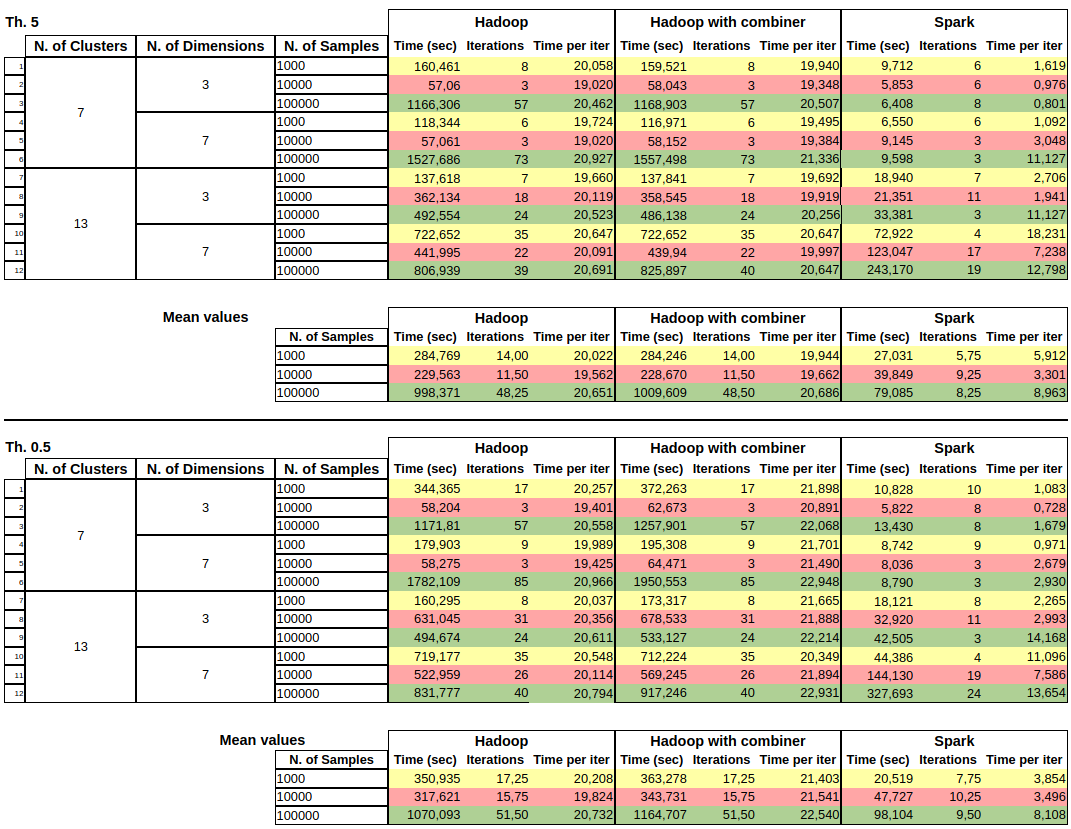
\includegraphics[width=1\textwidth]{images/tables}
\end{figure}\\
For each input file, the metrics we took into account to evaluate the performance are: the total execution time of the algorithms, the number of total iterations, and the average execution time per iteration. \\
We have noticed that, by introducing the Combiner class, performance has not significantly improved. Probably, this lack of improvement is due to the unreachability of some of our virtual machine during the execution of the tests with the Combiner.

\begin{figure}
\centering
\subfloat[]
{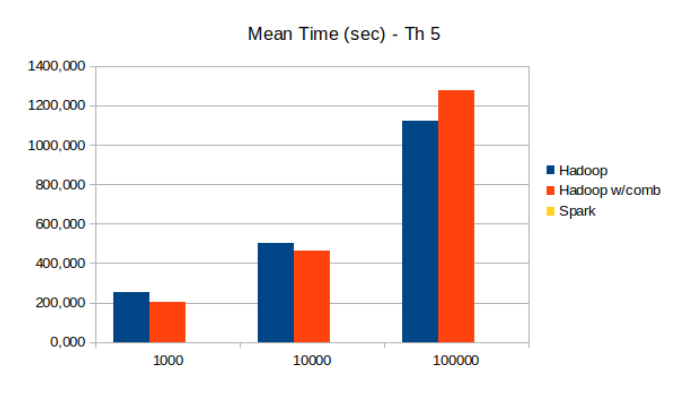
\includegraphics[width=.50\textwidth]{images/time_th5}}
\subfloat[]
{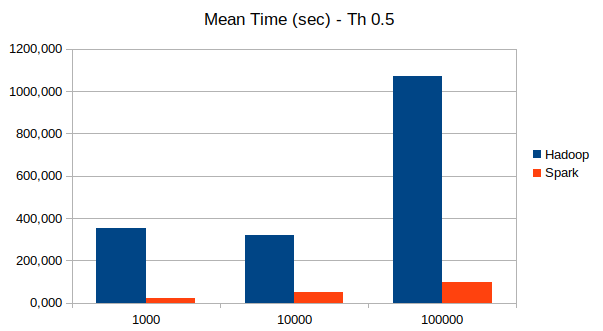
\includegraphics[width=.50\textwidth]{images/time_th05}} \\
\subfloat[]
{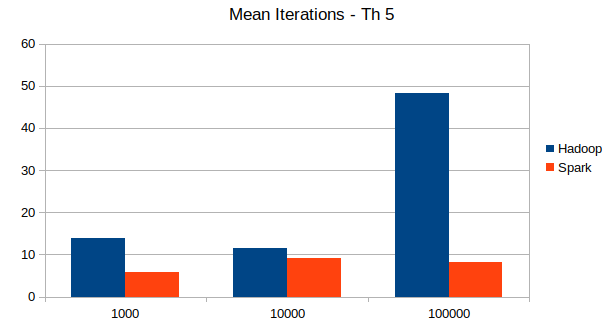
\includegraphics[width=.50\textwidth]{images/iter_th5}}
\subfloat[]
{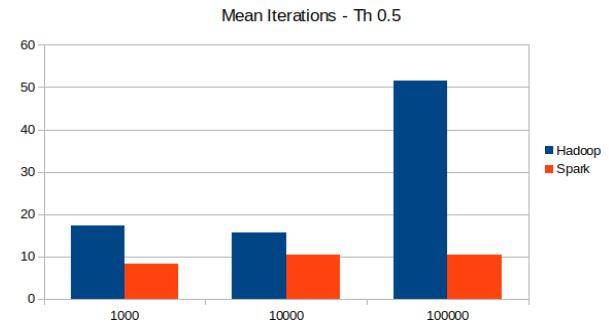
\includegraphics[width=.50\textwidth]{images/iter_th05}} \\
\subfloat[]
{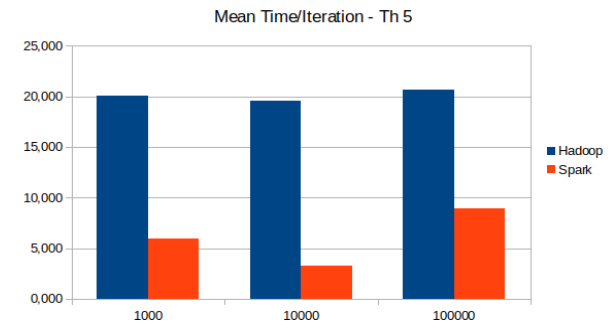
\includegraphics[width=.50\textwidth]{images/timexiter_th5}}
\subfloat[]
{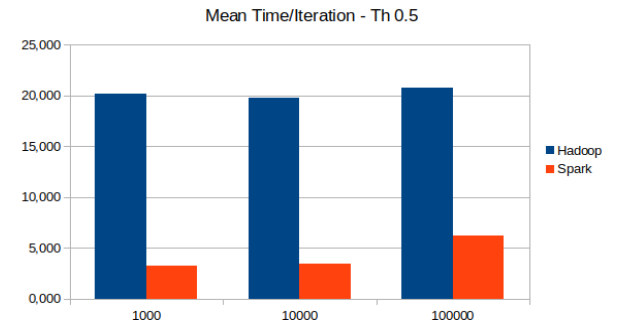
\includegraphics[width=.50\textwidth]{images/timexiter_th05}}\\
\end{figure}

\end{document}
